\chapter{ Challenges and Annotation Language Extension}
\section{Challenges and Idea}

To develop the system eclipse xtext, eclipse xtend and static analysis engine named smtcodan(which is developed in Java to detect C and C++ vulneribilities) are used. For building the source code annotation editor eclipse xtext is used. Modeling the source as UML Statechart opensource platform YAKINDU SCT editor is used. Inside YAKINDU sct editor to genrate the .c(c file) and .h(header file) eclipse xtend is used mainly for genrating code files from statechart. Let's see in briefly what is xtext, xtend and how it works.

\begin{itemize}	
	\item Xtext : Xtext is a framework for development of programming languages and domain specific languages.According to the \enquote{eclipse.org/Xtext}, it covers all aspects of a complete language infrastructure, from parsers, over linker, compiler or interpreter to fully-blown top-notch Eclipse IDE integration. It comes with great defaults for all these aspects which at the same time can be easily tailored to your individual needs.
	Here is an example of Xtext file:
		\begin{lstlisting}
		grammar org.xtext.example.mydsl.MyDsl with 
		org.eclipse.xtext.common.Terminals
		
		generate myDsl "http://www.xtext.org/example/mydsl/MyDsl"
		
		Model:
		messages+=Message*;
		
		Message:
		'Hello' name=ID '!';
		
		\end{lstlisting}
		 
	This language allows to write down a list of messages. The following would be proper input messages which are allowed to write:
		\begin{lstlisting}
			Hello User!
			Hello World!		
		\end{lstlisting}
	
	\item Xtend : According to the \enquote{eclipse.org/Xtend}, Xtend is a statically-typed programming language which translates to comprehensible Java source code. Syntactically and semantically Xtend has its roots in the Java programming language but improves on many aspects such as- Extension methods, Lambda Expressions, Active Annotations, Operator overloading, Powerful switch expressions, Multiple dispatch, Template expressions etc. Xtend has zero interoperability issues with Java: Everything you write interacts with Java exactly as expected. At the same time Xtend is much more concise, readable and expressive. Its small library is just a thin layer that provides useful utilities and extensions on top of the Java Development Kit (JDK). 
	Here is an example of Xtend file:
	\begin{lstlisting}
	package example	
	import java.util.List		
	class A {
	def greetToAll(List<String> names) {
		for(name: names) {
			println(name.helloMessage)
		}
	}
		
	def helloMessage(String name) {
		'Hello ' + name + '!'
		}
	}
	
	\end{lstlisting} 
	   
Xtend provides type inference, the type of name and the return types of the methods can be inferred from the context. Classes and methods are public by default, fields private. Semicolons are optional.
	
The example also shows the method helloMessage called as an extension method, like a feature of its first argument. Extension methods can also be provided by other classes or instances.
\end{itemize}


Previous annotation language grammer has been extended more
to detect implicit and explicit information flow bugs in UML
state charts and C code. The purpose of the same annotation language
can be used to add information flow constraints to UML state
charts and code in order to detect information flow errors.\\

The challenge was addressed by extending the annotation language containing textual annotations which can be used to annotate source code and UML state charts which are backward compatible.The single-line annotations have the same as previous consisting start tag "//@" and the multi-line annotations have the start tag "/*@" and the end tag "@*/" .\\

Some challenges throughout the approach are- converting textual
comments into annotations objects, introducing syntactically
correct annotations into files, how to use the same annotation
language in order to annotate UML state charts and source
code, dealing with scattered annotations and attaching annotations to the right function declaration or variable.\\

The eclipse xtext based grammar is used to parse the whole C/C++ language. The C/C++ source code file extensions (.h, .hh, .hhh, .hxx, .c, .cpp) and UML state chart annotation box (graphical boxes
which can be attached to different parts of a UML state chart diagram) can be annotated with policy language restrictions. The obtained CORE model (a one to one mapping from xtext grammar to the ECORE grammar representation) that can be reused for integrating the policy language into an UML state chart editor. Treating the annotation tags as EObjects created new possibilities for annotating
UML models.The policy language grammar has about 420 lines of code with code comments included. Source code generation is also supported by using
eclipse xtend, ANTLR and .mwe2 files. To parse other programming languages as well this annotation language parser can be used.The result is an extensible policy language and a highly reusable source code implementation as well as source code generator that can easily be used for annotating models and source files.

\section{Annotation Language Tags}
\begin{tabular}{l*{3}{c}r}
	\hline
	Annotation Type   & Annotation Tag & Description  \\
	\hline
	@function         & sink  		   & uses information \\
	                  & source         & source provides information	\\
	                  & authentication & authentication authenticates information	\\
	                  & declassification& declassification declassifies information	\\
	                  & sanitization   & sanitization sanitizes information	\\
	                  & trust\_boundary& trust\_boundary is a trust-boundary\\ \hline

	@parameter        & authenticated H/L & authenticated High/Low tags    \\
					  & declassified H/L  & declassified High/Low tags    \\
				      & sanitized H/L     & sanitized High/Low tags    \\ \hline
	@variable         & confidential H/L & confidential High/Low tags\\
					  & source H/L & source High/Low tags   \\
	\hline
\end{tabular}

\section{Language Implementation Process}

The process depicted in figure 3.1 was used in order to
implement annotation language. Figure 3.1 depicts the
annotation language implementation process. The process is
comprised of the following steps: At first, the .xtext file
containing the language grammar was extended following the requirements. Next the grammar file is compiled and software
artifacts are generated. After editing the .mwe2 file then compile it. The result of compiling is: a parser, a lexer and class bindings between these two (lexer and parser) and the grammar ECore model. The generated parser, lexer and the bindings were reused inside static analysis engine and in the UI source file editor. After opening and editing a source file with the editor,the file can be parsed and the annotations can be automatically loaded and used inside checkers.
\begin{figure}[htbp]
	\centering
	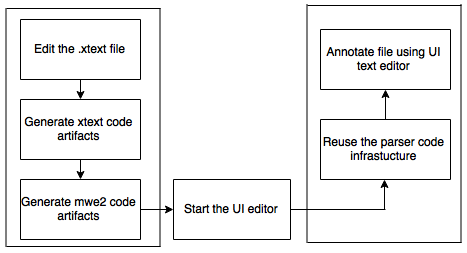
\includegraphics{styles/Language_Design_Process.png}
	\caption{Annotation language design process}
\end{figure}